\documentclass{standalone}
\usepackage{pgfplots}

\begin{document}
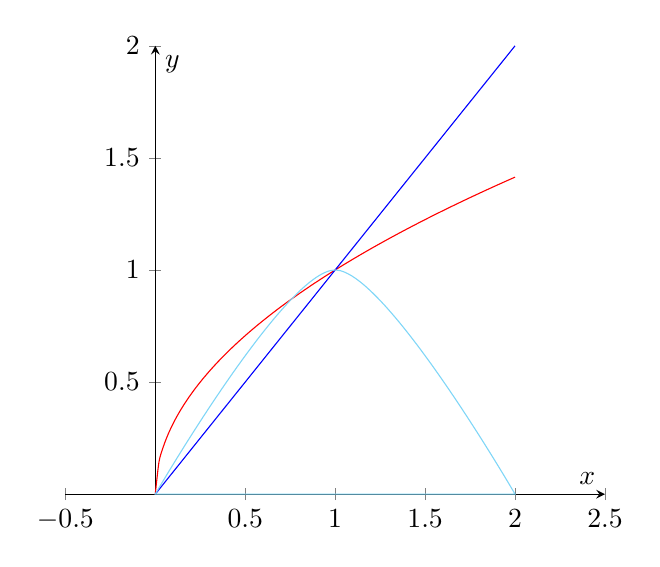
\begin{tikzpicture}
    \begin{axis}[
        axis lines = middle,
        xlabel = \(x\),
        ylabel = {\(y\)},
        ymin=0,
        ymax=2,
        xmin=-0.5,
        xmax=2.5,
        domain=0:2,
        samples=100,
        smooth,
        no markers,
        clip=false,
        ]
        \addplot [red] {sqrt(x)};
        \addplot [blue] {x};
        \addplot [cyan!50] coordinates {(0,0) (1,1) (2,0)} -- cycle;
    \end{axis}
\end{tikzpicture}
\end{document}